\documentclass{standalone}
\usepackage{tikz}
\usetikzlibrary{calc, angles, quotes}
\usepackage{amsfonts}
\linespread{1.5}

\begin{document}
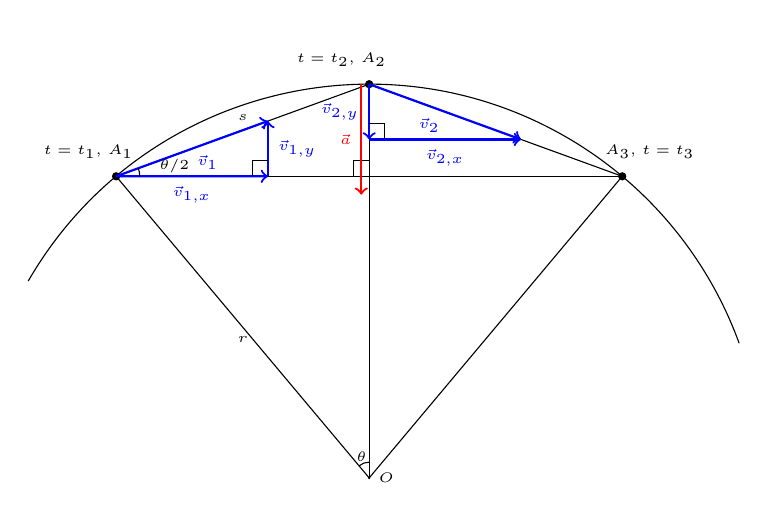
\begin{tikzpicture}
  \def\r{5.0};
  \def\ang{40};
  \coordinate (O) at (0.0, 0.0);
  \coordinate (A1) at ({-\r*sin(\ang)}, {\r*cos(\ang)});
  \coordinate (A2) at (0.0, {\r});
  \coordinate (A3) at ({\r*sin(\ang)}, {\r*cos(\ang)});
  \coordinate (K) at ({0}, {\r*cos(\ang)});
  \coordinate (K1) at ($(A1)!0.6!(K)$);
  \coordinate (K2) at ($(A1)!0.6!(A2)$);
  \coordinate (K3) at ($(A2)!0.6!(K)$);
  \coordinate (K4) at ($(A2)!0.6!(A3)$);
  \draw($(O)+(150:\r)$) arc (150:20:\r);
  \fill (O) circle[radius=0.5pt] node [right, font=\tiny] {$O$};
  \fill (A1) circle[radius=1.5pt] node [above, font=\tiny, xshift=-0.35cm, yshift=0.1cm] {$t=t_{1}$, $A_{1}$};
  \fill (A2) circle[radius=1.5pt] node [above, font=\tiny, xshift=-0.35cm, yshift=0.1cm] {$t=t_{2}$, $A_{2}$};
  \fill (A3) circle[radius=1.5pt] node [above, font=\tiny, xshift=0.35cm, yshift=0.1cm] {$A_{3}$, $t=t_{3}$};
  \draw (O)--(A1) node[midway, below, font=\tiny] {$r$};
  \draw (O)--(A2);
  \draw (O)--(A3);
  \draw (A1)--(A2) node[midway, above, font=\tiny] {$s$};
  \draw (A2)--(A3);
  \draw (A1)--(A3);
  \draw pic["$\theta$", font=\tiny, draw=black, angle radius=0.2cm, angle eccentricity=1.4] {angle=A2--O--A1};
  \draw pic[draw=black, angle radius=0.2cm, angle eccentricity=1.4] {right angle=A1--K--A2};
  \draw[->, thick, blue] (A1) -- ($(A1)!0.6!(A2)$) node[midway, below, font=\tiny, xshift=0.2cm, yshift=0.05cm]{$\vec{v}_{1}$};
  \draw[->, thick, blue] (A1) -- ($(A1)!0.6!(K)$) node[midway, below, font=\tiny]{$\vec{v}_{1, x}$};
  \draw[->, thick, blue] (K1) -- (K2) node[midway, right, font=\tiny]{$\vec{v}_{1, y}$};
  \draw[->, thick, blue] (A2) -- ($(A2)!0.6!(A3)$) node[midway, below, font=\tiny, xshift=-0.2cm, yshift=0.05cm]{$\vec{v}_{2}$};
  \draw pic[draw=black, angle radius=0.2cm, angle eccentricity=1.4] {right angle=A1--K1--K2};
  \draw[->, thick, blue] (A2) -- (K3) node[midway, left, font=\tiny]{$\vec{v}_{2, y}$};
  \draw[->, thick, blue] (K3) -- (K4) node[midway, below, font=\tiny]{$\vec{v}_{2, x}$};
  \draw pic[draw=black, angle radius=0.2cm, angle eccentricity=1.4] {right angle=A2--K3--K4};
  \draw pic["$\theta/2$", font=\tiny, draw=black, angle radius=0.3cm, angle eccentricity=2.5] {angle=K--A1--A2};
  \draw [->, thick, red] ($(A2)-(0.1, 0.0)$) -- ($($(A2)!1.2!(K)$)-(0.1, 0.0)$) node[midway, left, font=\tiny]{$\vec{a}$};
\end{tikzpicture}

\end{document}
